%==============================================================================
% Sjabloon onderzoeksvoorstel bachproef
%==============================================================================
% Gebaseerd op document class `hogent-article'
% zie <https://github.com/HoGentTIN/latex-hogent-article>

\documentclass{hogent-article}

% Invoegen bibliografiebestand
\usepackage[backend=biber]{biblatex}
\addbibresource{voorstel.bib}

% Informatie over de opleiding, het vak en soort opdracht
\studyprogramme{Professionele bachelor toegepaste informatica}
\course{Bachelorproef}
\assignmenttype{Onderzoeksvoorstel}

\academicyear{2025-2026}
\title{Optimalisatie van de Recovery Time Objective (RTO) in Active-Passive High Availability Clusters met Pacemaker en Corosync op RHEL-Nodes.}

\author{Arno Verhulst}
\projectrepo{https://github.com/vharno1612/bachelorproef-2526-vharno1612.git}
\email{arno.verhulst@student.hogent.be}


\supervisor[Co-promotor]{Dirk Allaert (oXya, \href{mailto:dallaert@oxya.com}{dallaert@oxya.com})}


% Binnen welke specialisatierichting uit 3TI situeert dit onderzoek zich?
% Kies uit deze lijst:
%
% - Mobile \& Enterprise development
% - AI \& Data Engineering
% - Functional \& Business Analysis
% - System \& Network Administrator
% - Mainframe Expert
% - Als het onderzoek niet past binnen een van deze domeinen specifieer je deze
%   zelf
%
\specialisation{System \& Network Administrator}
\keywords{Recovery Time Objective, High Availability, Webapplicatie, Pacemaker, Corosync, RHEL}

\begin{document}

\begin{abstract}
    Dit voorstel beschrijft een toegepast onderzoek gericht op de minimalisatie van de Recovery Time Objective (RTO) binnen een betaalbare Active-Passive High Availability (HA) webomgeving, gebouwd op Red Hat Enterprise Linux (RHEL)-compatibele nodes, gebruikmakend van de clusteringstechnologieën Pacemaker en Corosync. De centrale onderzoeksvraag luidt: \textit{“Hoe kan een betaalbare Active-Passive High Availability webomgeving, bestaande uit Pacemaker en Corosync op RHEL-compatibele nodes, geoptimaliseerd worden om de Recovery Time Objective (RTO) van de webapplicatie bij serveruitval te minimaliseren?”}. Het concrete doel van dit onderzoek is de ontwikkeling van een geoptimaliseerde Pacemaker-configuratie en een robuuste Power Fencing-implementatie, resulterend in een functionele proof-of-concept met een geminimaliseerde RTO, zodat de belangrijkste systemen van een bedrijf online blijven en de dienstverlening niet stilvalt. Door middel van een diepgaande literatuurstudie over de werking van Pacemaker, Corosync en STONITH, gekoppeld aan een iteratieve, experimentele methodologie (uitgevoerd in een virtuele omgeving, waarbij er de optie is om de oplossing later te valideren op de fysieke infrastructuur van het stagebedrijf), zullen de meest effectieve configuratieparameters worden geïdentificeerd en geoptimaliseerd. De verwachte resultaten omvatten een gevalideerde best-practice handleiding en een set optimale configuratiewaarden die de RTO opmerkelijk reduceren, wat een meerwaarde biedt voor IT-professionals die betaalbare, betrouwbare HA-oplossingen implementeren.
\end{abstract}

\tableofcontents

% De hoofdtekst van het voorstel zit in een apart bestand, zodat het makkelijk
% kan opgenomen worden in de bijlagen van de bachelorproef zelf.
%---------- Inleiding ---------------------------------------------------------

\section{Inleiding}%
\label{sec:inleiding}

De beschikbaarheid van vitale webapplicaties is een fundamentele vereiste voor hedendaagse organisaties. Ongeplande downtime als gevolg van serveruitval leidt niet alleen tot operationele verliezen, maar ook tot reputatieschade. Om de risico's op uitval te minimaliseren, is een High Availability (HA) cluster vandaag de dag noodzakelijk (een HA-cluster is een groep samenwerkende servers die redundant zijn geconfigureerd om bij het falen van één component de dienstverlening zonder merkbare onderbreking voort te zetten). De Recovery Time Objective (RTO) definieert de maximaal acceptabele tijd waarin een applicatie na een verstoring weer operationeel zou moeten zijn. Voor veel organisaties is een zo laag mogelijke RTO, bij voorkeur seconden, cruciaal.
\medskip

Dit onderzoek focust op Active-Passive HA-clusters op basis van Red Hat Enterprise Linux (RHEL)-compatibele systemen. Deze architectuur, die gebruikmaakt van de open-source componenten Pacemaker (als cluster resource manager) en Corosync (als lidmaatschapsservice), wordt gekozen vanwege zijn betaalbaarheid en robuustheid \autocite{RedHat2025}. De complexiteit van deze opstelling is echter de grootste uitdaging; de kern van dit onderzoek ligt dan ook in het finetunen van deze architectuur om te kunnen voldoen aan de strikte RTO-eisen van een moderne webdienst.
\medskip
    
Het onderzoek richt zich op IT-architecten, systeembeheerders en DevOps-engineers die verantwoordelijk zijn voor de implementatie en het beheer van Linux-gebaseerde infrastructuur en op zoek zijn naar betaalbare, open-source alternatieven voor commerciële HA-oplossingen. Eén specifiek doel is het ondersteunen van infrastructuurbedrijven die hun klanten een bewezen en geoptimaliseerde HA-webomgeving willen aanbieden.
\medskip
    
Hoewel Pacemaker en Corosync de basis voor HA leggen, is de standaardconfiguratie vaak niet geoptimaliseerd voor minimale RTO. Het bereiken van een RTO van enkele seconden vereist diepgaande kennis van de interne werking van Pacemaker en de interactie met essentiële componenten zoals STONITH (fencing). De hoofduitdaging is om, binnen de context van een betaalbare, open-source Active-Passive HA-oplossing, te identificeren welke parameters de failover het meest beïnvloeden en hoe deze geoptimaliseerd moeten worden om de RTO te minimaliseren.
\medskip
    
De hoofdonderzoeksvraag van dit onderzoek luidt als volgt:
\begin{quote}
    \textit{“Hoe kan een betaalbare Active-Passive High Availability webomgeving, bestaande uit Pacemaker en Corosync op RHEL-compatibele nodes, geoptimaliseerd worden om de Recovery Time Objective (RTO) van de webapplicatie bij serveruitval te minimaliseren?”}
\end{quote}
    
Het concrete eindresultaat is een functionele proof-of-concept (PoC) van de geoptimaliseerde Active-Passive HA-cluster, samen met een gedetailleerd technisch rapport en een best-practice handleiding. De PoC moet aantonen dat de RTO van de webdienst opmerkelijk gereduceerd is tot een zo laag mogelijke niveau. Dit omvat de implementatie van een robuust en betaalbaar Power Fencing-mechanisme (Power Fencing, specifiek STONITH, is een techniek waarbij een falende server fysiek wordt uitgeschakeld of herstart om te garanderen dat deze geen conflicterende acties meer uitvoert op het netwerk of de data), net zoals de realisatie van een set van geoptimaliseerde Pacemaker-configuratiewaarden die als blueprint kunnen dienen voor de doelgroep.

%---------- Stand van zaken ---------------------------------------------------

\section{Literatuurstudie}%
\label{sec:literatuurstudie}

De literatuurstudie is opgedeeld om zowel het theoretische probleemdomein (de werking van de HA-componenten en de factoren die de RTO bepalen) als het oplossingsdomein (de implementatie van STONITH en de RTO-optimalisatie\-pa\-ra\-me\-ters) te dekken.

\subsection{HA-Cluster Architectuur en RTO-Factoren (Probleemdomein)}

De kern van de onderzochte HA-oplossing wordt gevormd door de samenwerking tussen Pacemaker en Corosync. Corosync fungeert als de cluster lidmaatschapsservice, verantwoordelijk voor het doorgeven van statusberichten tussen de nodes via het netwerk en het detecteren van falende nodes. Pacemaker is de resource manager die, op basis van overeenkomsten met Corosync, beslist welke node welke resources (zoals een webdienst en een Virtual IP) moet beheren en initieert daarnaast ook de failover wanneer nodig \autocite{RedHatClusterWorkshop}.
\medskip

De Recovery Time Objective (RTO) is rechtstreeks afhankelijk van de tijd die nodig is voor overeenstemming en de daaropvolgende resource-migratie. Het akkoord over de status van de webdienst en het initiëren van een failover wordt sterk beïnvloed door de timeout waarden voor het stoppen, starten en monitoren van resources, net zoals de start-interval en resource-stickiness. Een te lage timeout kan leiden tot onnodige failovers; een te hoge waarde leidt tot een onacceptabel lange RTO \autocite{Clusterlabs2024}. Deelvragen met betrekking tot het probleemdomein pakken dit aan door te vragen naar:

\begin{itemize}
    \item Wat zijn de specifieke functies van Pacemaker, Corosync en STONITH (fencing) binnen de gekozen HA-architectuur, en hoe werken deze drie componenten samen om een consensus over de status van de webdienst te bereiken?
    \item Welke Pacemaker-configuratieparameters en constraints (zoals op-start-interval, resource-stickiness en timeout waarden) beïnvloeden het meest direct de snelheid van de failover en daarmee de RTO?
    \item Welke vereisten en risico's zijn cruciaal bij het gebruik van een virtueel IP-adres voor de webdienst in een Active-Passive cluster, en hoe beheert Pacemaker de migratie van dit virtuele IP om zero downtime bij failover te benaderen?
\end{itemize}

Pacemaker beheert de migratie van het virtuele IP-adres (gerepresenteerd door de IPaddr2 resource agent) door het van de falende node te verwijderen en op de nieuwe actieve node toe te voegen. Dit moet uiteraard zo snel mogelijk en betrouwbaar gebeuren om netwerkdowntime te minimaliseren en zero downtime bij failover te benaderen.

\subsection{Fencing en Optimalisatie (Oplossingsdomein)}

Fencing (STONITH) is cruciaal voor de data-integriteit in de cluster en het voorkomen van 'split-brain'-scenario's, waarbij twee nodes denken dat ze de controle hebben over een gedeelde resource \autocite{RedHatPolicies025}. STONITH ('Shoot The Other Node In The Head') zorgt ervoor dat een falende node van de resources wordt geïsoleerd, vaak door middel van Power Fencing. Voor een betaalbare oplossing is de implementatie van een geschikte fence\_agent, zoals fence\_ipmilan (indien IPMI beschikbaar is) of een ander betaalbaar mechanisme, essentieel \autocite{Beekhof2025, RedHat2025}.
\medskip

De minimalisatie van de RTO vereist een specifieke optimalisatiemethode. De meest directe invloed op de RTO ligt in de timeout en retry waarden voor de resource-agents. Het aanpassen van de resource-stickiness beïnvloedt de failback-beslissing en kan de uiteindelijke stabiliteit verbeteren. Literatuur toont aan dat een stapsgewijze, experimentele aanpak noodzakelijk is om de perfecte balans te vinden tussen failover-snelheid en stabiliteit van de cluster \autocite{Robert2025}.
\medskip

De deelvragen met betrekking tot het oplossingsdomein zijn:
\begin{itemize}
    \item Hoe kan een robuust en betaalbaar Power Fencing-mechanisme (STONITH), - cruciaal voor het garanderen van data-integriteit -  effectief geïmplementeerd en getest worden met behulp van een geschikte fence agent om 'split-brain'-scenario's betrouwbaar te voorkomen?
    \item Wat is de gemeten gemiddelde Recovery Time Objective (RTO) van de webdienst, gesimuleerd voor ten minste drie verschillende uitvalscenario's (bijvoorbeeld een harde node-crash, een service crash, en netwerkisolatie)?
    \item Hoe kan de initiële Pacemaker-configuratie, op basis van de theoretisch geïdentificeerde parameters, stapsgewijs geoptimaliseerd worden om de RTO tot het laagst mogelijke niveau te reduceren, en wat is de impact van deze optimalisatie op de normale performantie van de webdienst?
\end{itemize}

%---------- Methodologie ------------------------------------------------------
\section{Methodologie}%
\label{sec:methodologie}

De methodologie hanteert een experimenteel onderzoeksontwerp met een duidelijke focus op de technische implementatie en kwantitatieve meting. De aanpak wordt onderverdeeld in drie fasen, waarbij de antwoorden op de deelvragen voor het probleem- en oplossingsdomein worden verzameld.

\begin{figure}[htbp]
    \centering
    \resizebox{0.5\textwidth}{!}{
        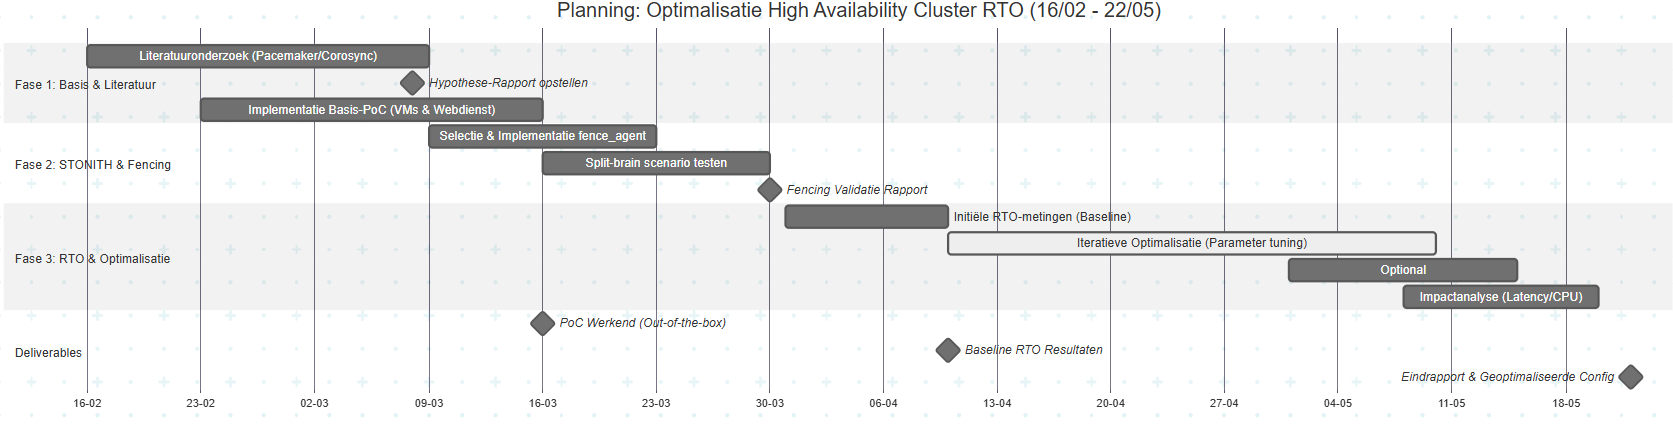
\includegraphics{gantt.png}
    }
    \caption{Gantt Chart Projectplanning}
    \label{fig:gantt_chart}
\end{figure}

\subsection{Fase 1: Basissysteem en Literatuuronderzoek}
Deze eerste fase legt de basis voor het onderzoek en beantwoordt de theoretische deelvragen over het probleemdomein.
\medskip

We starten met een diepgaand literatuuronderzoek. Hierbij wordt de officiële documentatie en relevante vakliteratuur over Pacemaker, Corosync en STONITH uitgebreid bestudeerd. Het doel is om niet alleen de exacte werking van deze tools te ontdekken, maar vooral om de invloed van configuratieparameters op de failover time in kaart te brengen. Dit levert ons een essentieel rapport op over welke RTO-parameters naar verwachting de grootste invloed zullen hebben op de hersteltijd.
\medskip

Vervolgens implementeren we de basis Proof-of-Concept (PoC). De Active-Passive cluster wordt opgezet op twee virtuele machines draaiend op Red Hat Enterprise Linux 9. Deze machines worden uitgerust met Pacemaker en Corosync en een standaard webdienst (bijvoorbeeld Apache of NGINX) wordt geconfigureerd als een gedeelde clusterresource, inclusief een virtueel IP-adres. De initiële configuratie volgt hierbij de aanbevolen, nog niet geoptimaliseerde, 'out-of-the-box' instellingen.

\subsection{Fase 2: Implementatie en Validatie van STONITH}
Het Power Fencing-mechanisme is cruciaal; zonder een STONITH-oplossing is betrouwbare HA onmogelijk.
\medskip

We richten ons op een betaalbare STONITH-implementatie door een geschikte fence\_agent te selecteren. We maken gebruik van de fence\_ipmilan agent of de API-gebaseerde agent van het aanwezige virtualisatieplatform.
\medskip

Vervolgens testen we dit grondig. Door een 'split-brain'-situatie na te bootsen, valideren we de betrouwbaarheid van de Fencing. Dit wordt vastgelegd in een helder Fencing Validatie Rapport.

\subsection{Fase 3: RTO-Meting en Iteratieve Optimalisatie}
Dit is het hart van het onderzoek: het meten en optimaliseren van de hersteltijd op de infrastructuur van het stagebedrijf oXya.
\medskip

De PoC-omgeving is opgezet op een dedicated cluster bij oXya, waarbij twee virtuele nodes draaien op Red Hat Enterprise Linux 9. Elke node beschikt over voldoende RAM en vCPUs om een realistische belasting te simuleren. Voor Power Fencing wordt gebruikgemaakt van een agent die communiceert met de fysieke beheerkaarten (zoals IPMI) van de onderliggende hosts of de API van het virtualisatieplatform.
\medskip

Om de RTO exact en objectief vast te leggen, wordt gebruikgemaakt van een externe monitoring- en logging-node. De volgende instrumenten worden ingezet:

\begin{itemize}
    \item HTTP Probing (Availability): Een script op basis van cURL of een tool zoals Uptime Kuma voert elke 500ms een request uit naar het Virtueel IP. De tijd tussen het eerste gefaalde request en het eerste succesvolle herstel na de failover definieert de bruto RTO.
    \item Pacemaker Logging \& Crm\_mon: De interne logs van de cluster worden geanalyseerd met journalctl om de exacte tijdstippen van failure detection, fencing execution en resource start tot op de milliseconde te synchroniseren.
    \item Wireshark/Tcpdump: Voor de analyse van de netwerkmigratie wordt netwerkverkeer onderschept om te meten hoe lang de ARP-verversing duurt voordat de switch het verkeer naar de nieuwe node stuurt.
\end{itemize}

Eerst wordt een nulmeting uitgevoerd op de basisconfiguratie voor drie scenario's: een harde servercrash, een service-crash en netwerkisolatie. Vervolgens start de iteratieve optimalisatie waarbij parameters zoals timeout-waarden, het start-interval en de resource-stickiness stapsgewijs worden aangepast. Na elke wijziging worden de metingen herhaald om de impact op de RTO en de systeemstabiliteit te valideren.


%---------- Verwachte resultaten ----------------------------------------------
\section{Verwacht resultaat, conclusie}%
\label{sec:verwachte_resultaten}

De uitkomsten van dit onderzoek geven antwoord op de opgestelde deelvragen en vormen de kern van de bachelorproef. Het belangrijkste resultaat is een zorgvuldig geteste set van configuratieparameters, waarbij de nadruk ligt op de finetuning van timeout-waarden en resource-stickiness. De verwachting is dat deze optimalisaties de $RTO$ met minstens 50\% kunnen reduceren in vergelijking met de standaardinstellingen van een RHEL-cluster. De streefwaarden voor de verschillende uitvalscenario's worden overzichtelijk samengevat in Tabel~\ref{tab:verwachte_rto}. Deze waarden zijn gebaseerd op verschillende vakliteratuur en zijn uitermate realistisch.

\begin{table}[h]
    \centering
    \caption{Verwachte RTO-metingen bij geoptimaliseerde configuratie. \autocite{JWBSystems}, \autocite{OracleC}}
    \label{tab:verwachte_rto}
    \resizebox{\columnwidth}{!}{%
        \begin{tabular}{|l|c|c|}
            \hline
            \textbf{Uitvalscenario} & \textbf{Standalone RTO} & \textbf{HA Geoptimaliseerd (RTO)} \\
            \hline
            Harde Node Crash        & Minuten tot uren        & 30 -- 60 seconden* \\
            Service / Software Crash & Minuten tot uren        & Seconden tot minuten \\
            Netwerkisolatie         & Minuten tot uren        & < 60 seconden \\
            \hline
        \end{tabular}%
    }
\end{table}
\medskip

Naast de reductie van de hersteltijd, wordt een STONITH-mechanisme gerealiseerd dat zowel robuust als kosteneffectief is. In de testfase zal worden aangetoond dat deze methode 'split-brain'-situaties betrouwbaar uitsluit, wat belangrijk is voor de integriteit van de webapplicatie. Door middel van een kwantitatieve analyse worden de exacte hersteltijden bij verschillende storingsscenario's in kaart gebracht, wat het bewijs levert voor de effectiviteit van de gekozen instellingen.
\medskip

De uiteindelijke conclusie van dit werk zal aantonen dat een zeer hoge beschikbaarheid niet afhankelijk hoeft te zijn van dure commerciële software. Door een gedisciplineerde configuratie van Pacemaker en een doordachte STONITH-implementatie wordt de haalbaarheid van een snelle, betaalbare Active-Passive HA-omgeving bewezen. De fundamentele meerwaarde voor IT-professionals en de infrastructuursector zit in de praktische blueprint die dit onderzoek oplevert. Dit onderzoek dient als een blueprint om bedrijfskritieke diensten betrouwbaarder te maken en de continuïteit te waarborgen met open-source middelen.

\autocite{Clusterlabs2024}



\printbibliography[heading=bibintoc]

\end{document}
